% prelab2
\documentclass{IEEEtran}
\usepackage{booktabs}
\usepackage{graphicx}
\usepackage{fancyhdr}
\usepackage{framed}
\usepackage{siunitx}
\pagestyle{fancy}
\lhead{}
\chead{}
\rhead{}
\lfoot{}
\cfoot{}
\rfoot{\thepage}
\title{Prelab 2 Amplifiers}
\author{Group 8: Muhan Li \and Man Sun \and Mingxiao An \\ EE233 Circuit Theory}
\IEEEaftertitletext{\centering \vspace{-10pt} \fontsize{11}{11}\textsc{Department of Electrical Engineering, University of Washington, Seattle, WA, 98195} \vspace{10pt}}

\begin{document}
	
	\maketitle
	
	\section{\textbf{Prelab\#1}}
	The typical values of parameters of \textit{LM148} are shown in table[\ref{tab:pl1}], figure[\ref{fig:101}], and figure[\ref{fig:102}].
	
	\begin{table}[!htbp]
		\centering
		\caption{The typical values of parameters}
		\begin{tabular}{lcl}
			\toprule
			Parameter & value & \\
			\midrule
			Power supplies & $\pm22\si{V}$ & \\
			Input resistance & $2.5\si{M\Omega}$ & \\
			Slew rate & $0.5\si{V/\mu s}$ & \\
			\bottomrule
		\end{tabular}
		\label{tab:pl1}
	\end{table}
	
	\begin{figure}[!htbp]
		\centering
		\begin{framed}
			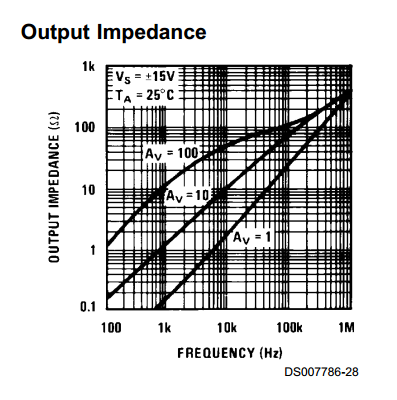
\includegraphics[width=\linewidth]{images/1_1.PNG}
			\caption{Output impedance}
		\end{framed}
		\label{fig:101}
	\end{figure}
	
	\begin{figure}[!htbp]
		\centering
		\begin{framed}
			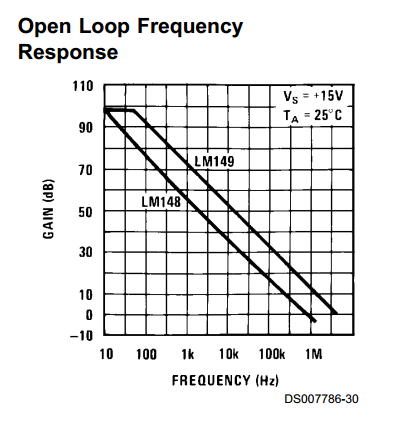
\includegraphics[width=\linewidth]{images/1_2.PNG}
			\caption{Open-loop voltage gain}
		\end{framed}
		\label{fig:102}
	\end{figure}
	
	\section{\textbf{Prelab\#2}}
	\begin{equation}
		\mathrm{gain} = \frac{V_{\mathrm{out}}}{V_{\mathrm{in}}} = 1
	\end{equation}
	
	\section{\textbf{Prelab\#3}}
	\subsection{Calculate the time}
	\begin{equation}
		t = \frac{\Delta V}{\mathrm{SlewRate}}
		= \frac{10\si{V}-(-10\si{V})}{0.5\si{V/\mu s}} = 40\si{\mu s}
	\end{equation}
	\subsection{Result comparison}
	The time we read from the datasheet is the gap between the two yellow dots on figure[\ref{fig:301}]. It is $40\si{ms}$, so we have no error. Temperatures, or input resistance, can contribute to error between the theoretical value and actual value.
	\begin{figure}[!htbp]
		\centering
		\begin{framed}
			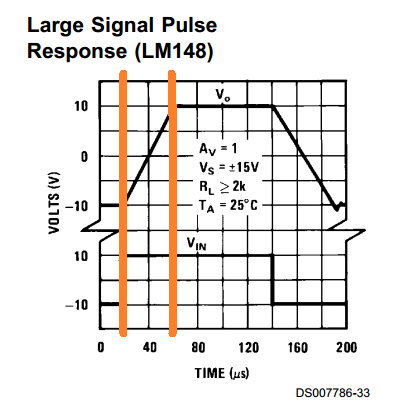
\includegraphics[width=\linewidth]{images/3_1.PNG}
			\caption{Open-loop voltage gain}
		\end{framed}
		\label{fig:301}
	\end{figure}
	
	\section{\textbf{Prelab\#4}}
	\section{\textbf{Prelab\#5}}
	\section{\textbf{Prelab\#6}}
	\section{\textbf{Prelab\#7}}
	\section{\textbf{Prelab\#8}}
	\section{\textbf{Prelab\#9}}
	\section{\textbf{Prelab\#10}}
	\section{\textbf{Prelab\#11}}
\end{document}

